\section*{\fontsize{16}{14}\selectfont Aim: Usage of OpenProj or similar software to draft plan and to track the progress of a project.}

The OpenProj free project management tool has now been superceded by ProjectLibre. The new program is also free for any use and is based on OpenProj. Project managers can use OpenProj, a free task tracking application, when creating effective plans\\
The best way to understand how a project plan may be created using OpenProj is to study a realistic example such as the one below.\\\\
From the graphical presentation of the critical path, to resource balancing and task elaboration, OpenProj gives the project manager a set of functions that help to monitor project performance.\\\\
To create projects in OpenProj Software:
\begin{enumerate}

\item Having downloaded and installed the OpenProj software; start OpenProj from the start menu of Windows or via the icon on your desktop. After the license agreement, OpenProj starts with a choice of creating a new project or opening an existing one. Choose Create Project.



\item Enter a name for the project, the project manager's name and a start date (which can also be modified later if required). Provide a description in the Notes section as you see fit.

\item The application window will be displayed consisting of following main components:- 
\begin{itemize}
\item{Indicator Column}:- In this column, symbols are displayed to show the status of the corresponding tasks (see right). 

\item{Task Number Column}:- Task numbers are assigned by OpenProj automatically when data is entered. The user does not enter information into this box. 

\item{Time Scale}:- In many views, OpenProj shows a timeline whose scale can be changed via the + and - magnifying glass icon on the menu above. 

\item{Information View Type}:- The area along the left side of the window lists a number of buttons representing the available views. Gantt, Network, Resources, WBS (work breakdown structure), RBS (resource breakdown structure), Reports, Task Usage and Resource Usage.  
\end{itemize}
\end{enumerate}
The lower view buttons open a split-screen where resource mapping tables and resource utilization as a graphic can be displayed. You can toggle views on and off by clicking the same button repeatedly.
\begin{itemize}
\item \textbf{Gantt Chart }
A Gantt chart, commonly used in project management, is one of the most popular and useful ways of showing activities (tasks or events) displayed against time. On the left of the chart is a list of the activities and along the top is a suitable time scale. Each activity is represented by a bar; the position and length of the bar reflects the start date, duration and end date of the activity. This allows you to see at a glance: 
What the various activities are?
When each activity begins and ends?
\begin{figure}[!ht]
\centering
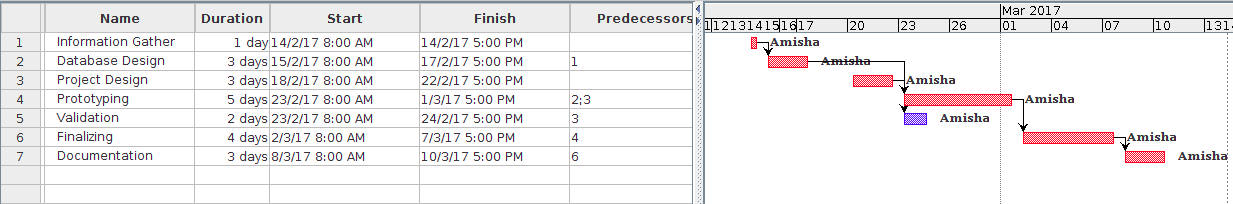
\includegraphics[width=1\linewidth]{input/images/am_gantt.png}
\label{fig:image1}
\caption{Gantt chart}
\end{figure}

\item\textbf{ Network Chart}
A network diagram is essentially a flow chart that includes all of the project elements and how they relate to one another. It shows parallel activities and the links between each activity. Network logic is the collection of activity dependencies that make up a network diagram for a particular project. In other words, certain tasks are dependent on one another to complete the project. This creates a logical stream of events that will lead to completion of the project.

\begin{figure}[!ht]
\centering
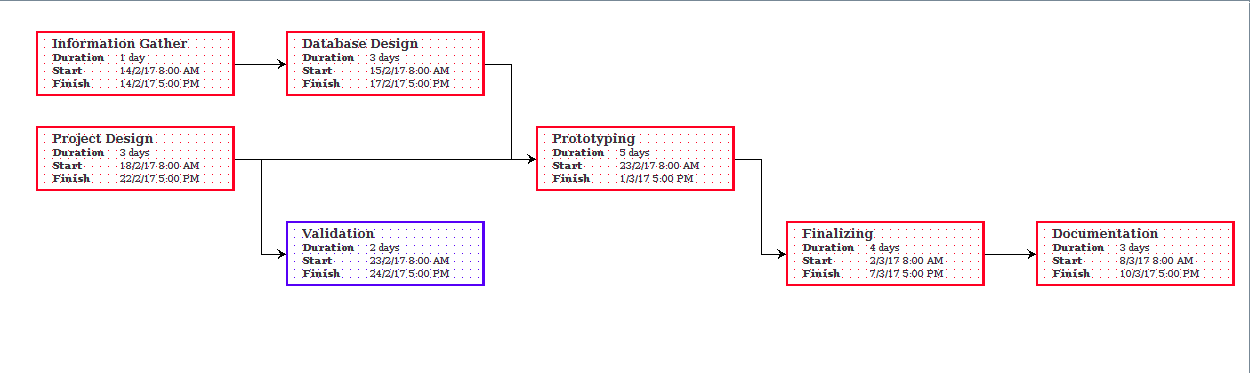
\includegraphics[width=1\linewidth]{input/images/am_ne.png}
\label{fig:image1}
\caption{Network chart}
\end{figure}

\item \textbf{Work Breakdown Structure(WBS)}
A work breakdown structure (WBS),in project management and system engineering, is a deliverable-oriented decomposition of a project into smaller components.A work breakdown structure is a key project deliverable that organizes the team's work into manageable sections. The Project Management Body of Knowledge defines the work breakdown structure as a "A hierarchical decomposition of the total scope of work to be carried out by the project team to accomplish the project objectives and create the required deliverables."
A work breakdown structure element may be a product,data,service or any combination thereof. A WBS also provides the necessary framework for detailed cost estimating and control along with providing guidance for schedule development and control.

\begin{figure}[!ht]
\centering
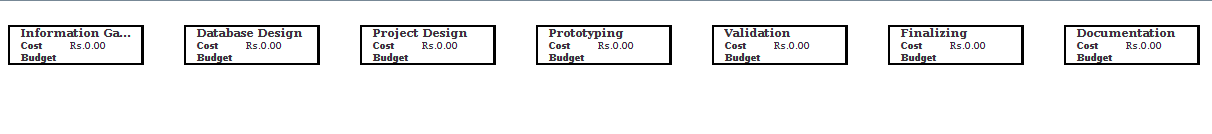
\includegraphics[width=1\linewidth]{input/images/am_wbs.png}
\label{fig:image1}
\caption{Work Breakdown Structure}
\end{figure}

\item \textbf{Reverse Breakdown Structure(RBS)}
The resource breakdown structure (RBS) is a hierarchical list of resources related by function and resource type that is used to facilitate planning and controlling of project work. The Resource Breakdown Structure includes, at a minimum, the personnel resources needed for successful completion of a project, and preferably contains all resources on which project funds will be spent, including personnel, tools, machinery, materials, equipment and fees and licenses.

\begin{figure}[!ht]
\centering
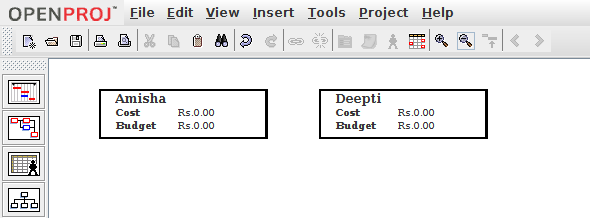
\includegraphics[width=1\linewidth]{input/images/am_rbs.png}
\label{fig:image1}
\caption{Reverse Breakdown Structure}
\end{figure}

\item \textbf{Histogram }
A histogram is a chart type that shows data distribution and it can help in estimating the distribution probability of a variable.

\begin{figure}[!ht]
\centering
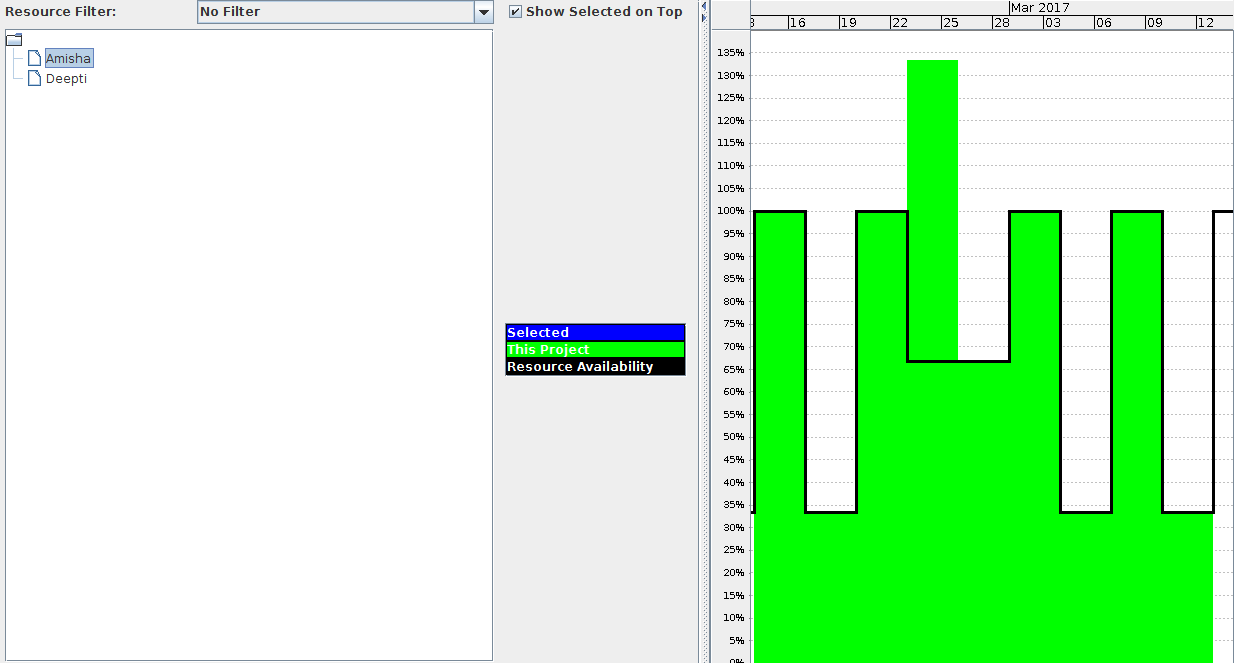
\includegraphics[width=0.8\linewidth]{input/images/am_histogram.png}
\label{fig:image1}
\caption{Histogram}
\end{figure}



\begin{figure}[!ht]
\centering
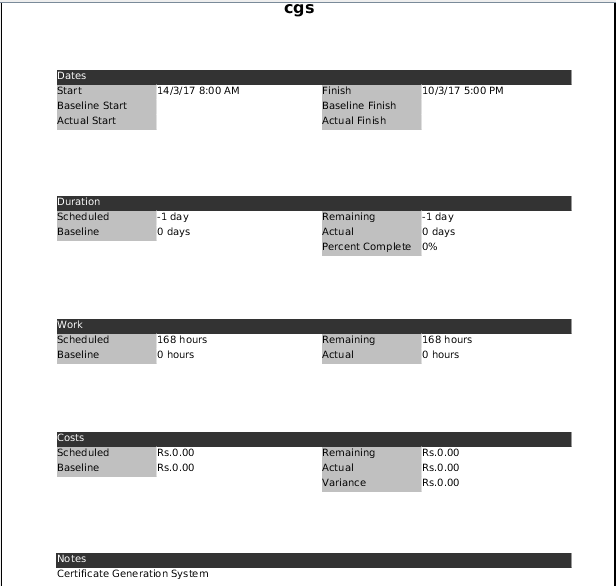
\includegraphics[width=0.8\linewidth]{input/images/am_reports.png}
\label{fig:image1}
\caption{Report Chart}
\end{figure}


\begin{figure}[!ht]
\centering
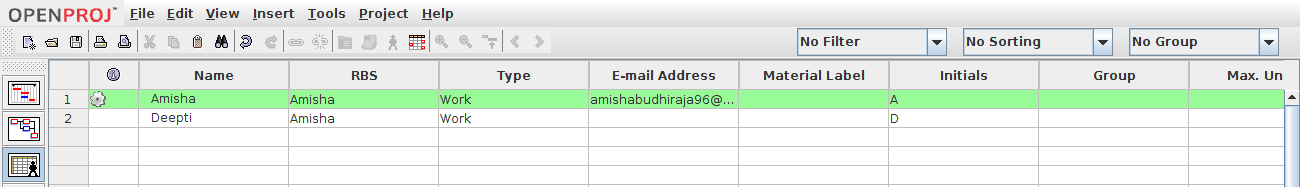
\includegraphics[width=1\linewidth]{input/images/am_resources.png}
\label{fig:image1}
\caption{Resources}
\end{figure}


\begin{figure}[!ht]
\centering
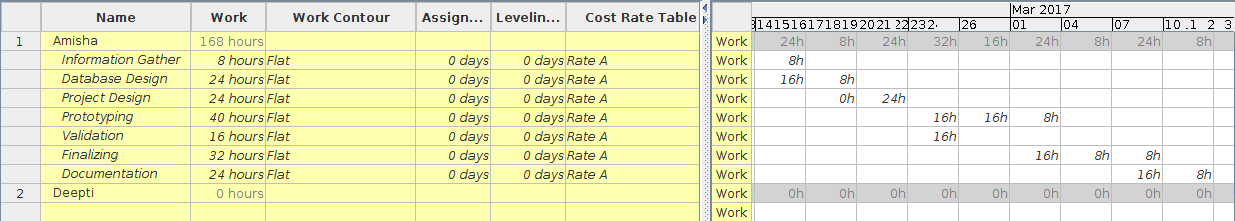
\includegraphics[width=1\linewidth]{input/images/am_res_usage.png}
\label{fig:image1}
\caption{Resource Usage}
\end{figure}



\begin{figure}[!ht]
\centering
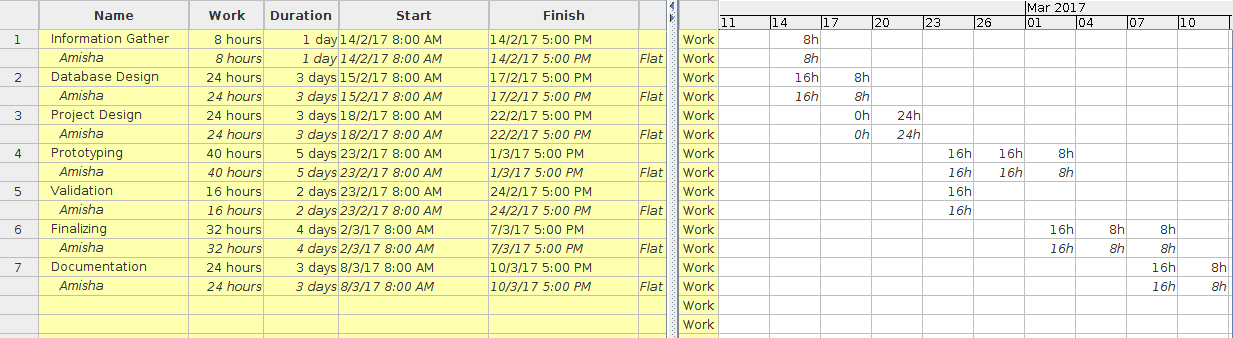
\includegraphics[width=1\linewidth]{input/images/am_task_usage.png}
\label{fig:image1}
\caption{Task Usage}
\end{figure}
\end{itemize}
